\documentclass[english,a4paper,12pt,oneside]{article}


%\includeonly{lab4}

%Drafting options
%uncomment for double spacing
%\doublespacing

% \usepackage{acronym}
\usepackage{times}
\usepackage{setspace} 
\usepackage{amsmath}    % need for subequations
\usepackage{graphicx}   % need for figures
%\usepackage{picture}
% \usepackage{wrapfig}
\usepackage{graphics}
 \graphicspath{{./}{../data/}}
 \usepackage{epstopdf}
\usepackage{color}
\usepackage{listings}
\lstset{basicstyle=\ttfamily\footnotesize,
	breaklines=true,
%    basicstyle=\ttfamily,
    keywordstyle=\color{blue}\ttfamily,
    stringstyle=\color{red}\ttfamily,
    commentstyle=\color{magenta}\ttfamily,
%    morecomment=[l][\color{magenta}]{\#}
}
\usepackage{verbatim}   % useful for program listings
\usepackage{color}      % use if color is used in text
\usepackage{subfigure}  % use for side-by-side figures
\usepackage{varioref}
\usepackage{anysize}
\usepackage{natbib}
\usepackage{fancyhdr}
% \usepackage{units}
\usepackage{longtable}
%\usepackage{bbding}
%\usepackage{aeguill}
\usepackage[hyphens]{url}
\usepackage{hyperref}

\setlength{\parskip}{8pt plus 2pt minus 2pt}
\setlength{\parindent}{0pt}

\marginsize{2cm}{2cm}{2cm}{2cm}
\fancypagestyle{plain}{%
  \fancyhf{}%
  \renewcommand{\headrulewidth}{0pt}%
  \renewcommand{\footrulewidth}{0pt}%
}

\pagestyle{fancy}
%\renewcommand{\sectionmark}[1]{\markright{\thesection.\ #1}}

\renewcommand{\sectionmark}[1]{\markright{#1}{}}
\renewcommand{\subsectionmark}[1]{\markright{#1}{}}
\renewcommand{\subsubsectionmark}[1]{\markright{#1}{}}

%\renewcommand{\quote}[1]{\textit{\begin{quote}#1\end{quote}}}
\newcommand{\bold}[1]{\emph{\textbf{#1}}}

\newcommand{\varentry}[1]{{\guillemotleft}\emph{#1}{\guillemotright}}
\newcommand{\code}[1]{{\tt #1}}

\headheight 10mm


\rhead{05/02/2019}
\chead{}
\lhead{ICP3038 --- Computer Vision}
\rfoot{}
\cfoot{- \thepage  \,\,-}
\lfoot{}

\renewcommand{\headrulewidth}{0.4pt}
\renewcommand{\footrulewidth}{0.4pt} 



%%%%%%%%%%%%%%%%%%%%%%%%%%%%%%%%%%%%%%%%%%%%%%%%%%%%%%%%%%%%%%%%%%%%%%%%%%%%%%%%
\begin{document}

\sloppy 

%%%%%%%%%%%%%%%%%%%%%%%%%%%%%%%%%%%%%%%%%%%%%%%%%%%%%%%%%%%%%%%%%%%%%%%%%%%%%%%%
\section*{Laboratory 8: Edge detection / Basic GUI / Displaying several images in the same window}

\null\vfill
The aims of today's lab are:
\begin{itemize}
	\item Add sliders to our windows;
	\item Displaying several images next to each other.
	\item Use the Canny operator.
%  	\item Investigate how to use a video stream (camera or file) (self-study).
\end{itemize}
In short, you are going to write parts of the demo programs seen during the lecture.

To achieve these goals, we will create several programs:
\begin{enumerate}
	\item \verb+edgeDetection1.cxx+: A simple program using OpenCV to detect edges;
	\item \verb+edgeDetection2.cxx+: We will improve the functionalities of the previous program to make it interactive;
	\item \verb+edgeDetection3.cxx+: We will improve edge detection using a Canny operator.
% 	\item \verb+edgeVideo.cxx+: Same as the previous program, but using a video stream.
\end{enumerate}
You are provided with the skeletons and a \verb+CMakeLists.txt+  file in the \verb+src+ directory. 
% You can add the two programs to the \verb+CMakeLists.txt+ file from last week (or use the new one provided).

Everything we did last week is relevant to today's session. 
You are expected to have completed Lab 7~already. 
You are also expected to look for information on OpenCV's website if needed. 
The lab script provides a good starting point. 
Additional information can be found at \url{http://docs.opencv.org/master/d4/d86/group__imgproc__filter.html}.
\vfill\null

%%%%%%%%%%%%%%%%%%%%%%%%%%%%%%%%%%%%%%%%%%%%%%%%%%%%%%%%%%%%%%%%%%%%%%%%%%%%%%%%
\newpage
\section{Edge Detection using Scharr and Thresholding}

We will write the code in \verb+edgeDetection1.cxx+.
The program takes two arguments from the command line:
\begin{itemize}
 \item The input file (\verb+argv[1]+); 
 \item The output file (\verb+argv[2]+).
\end{itemize}

\subsection{Main Steps}
The overall flow chart corresponding to the program is given in Figure~\ref{fig:flowChart}. 
\begin{figure}[htbp]
 \centering
 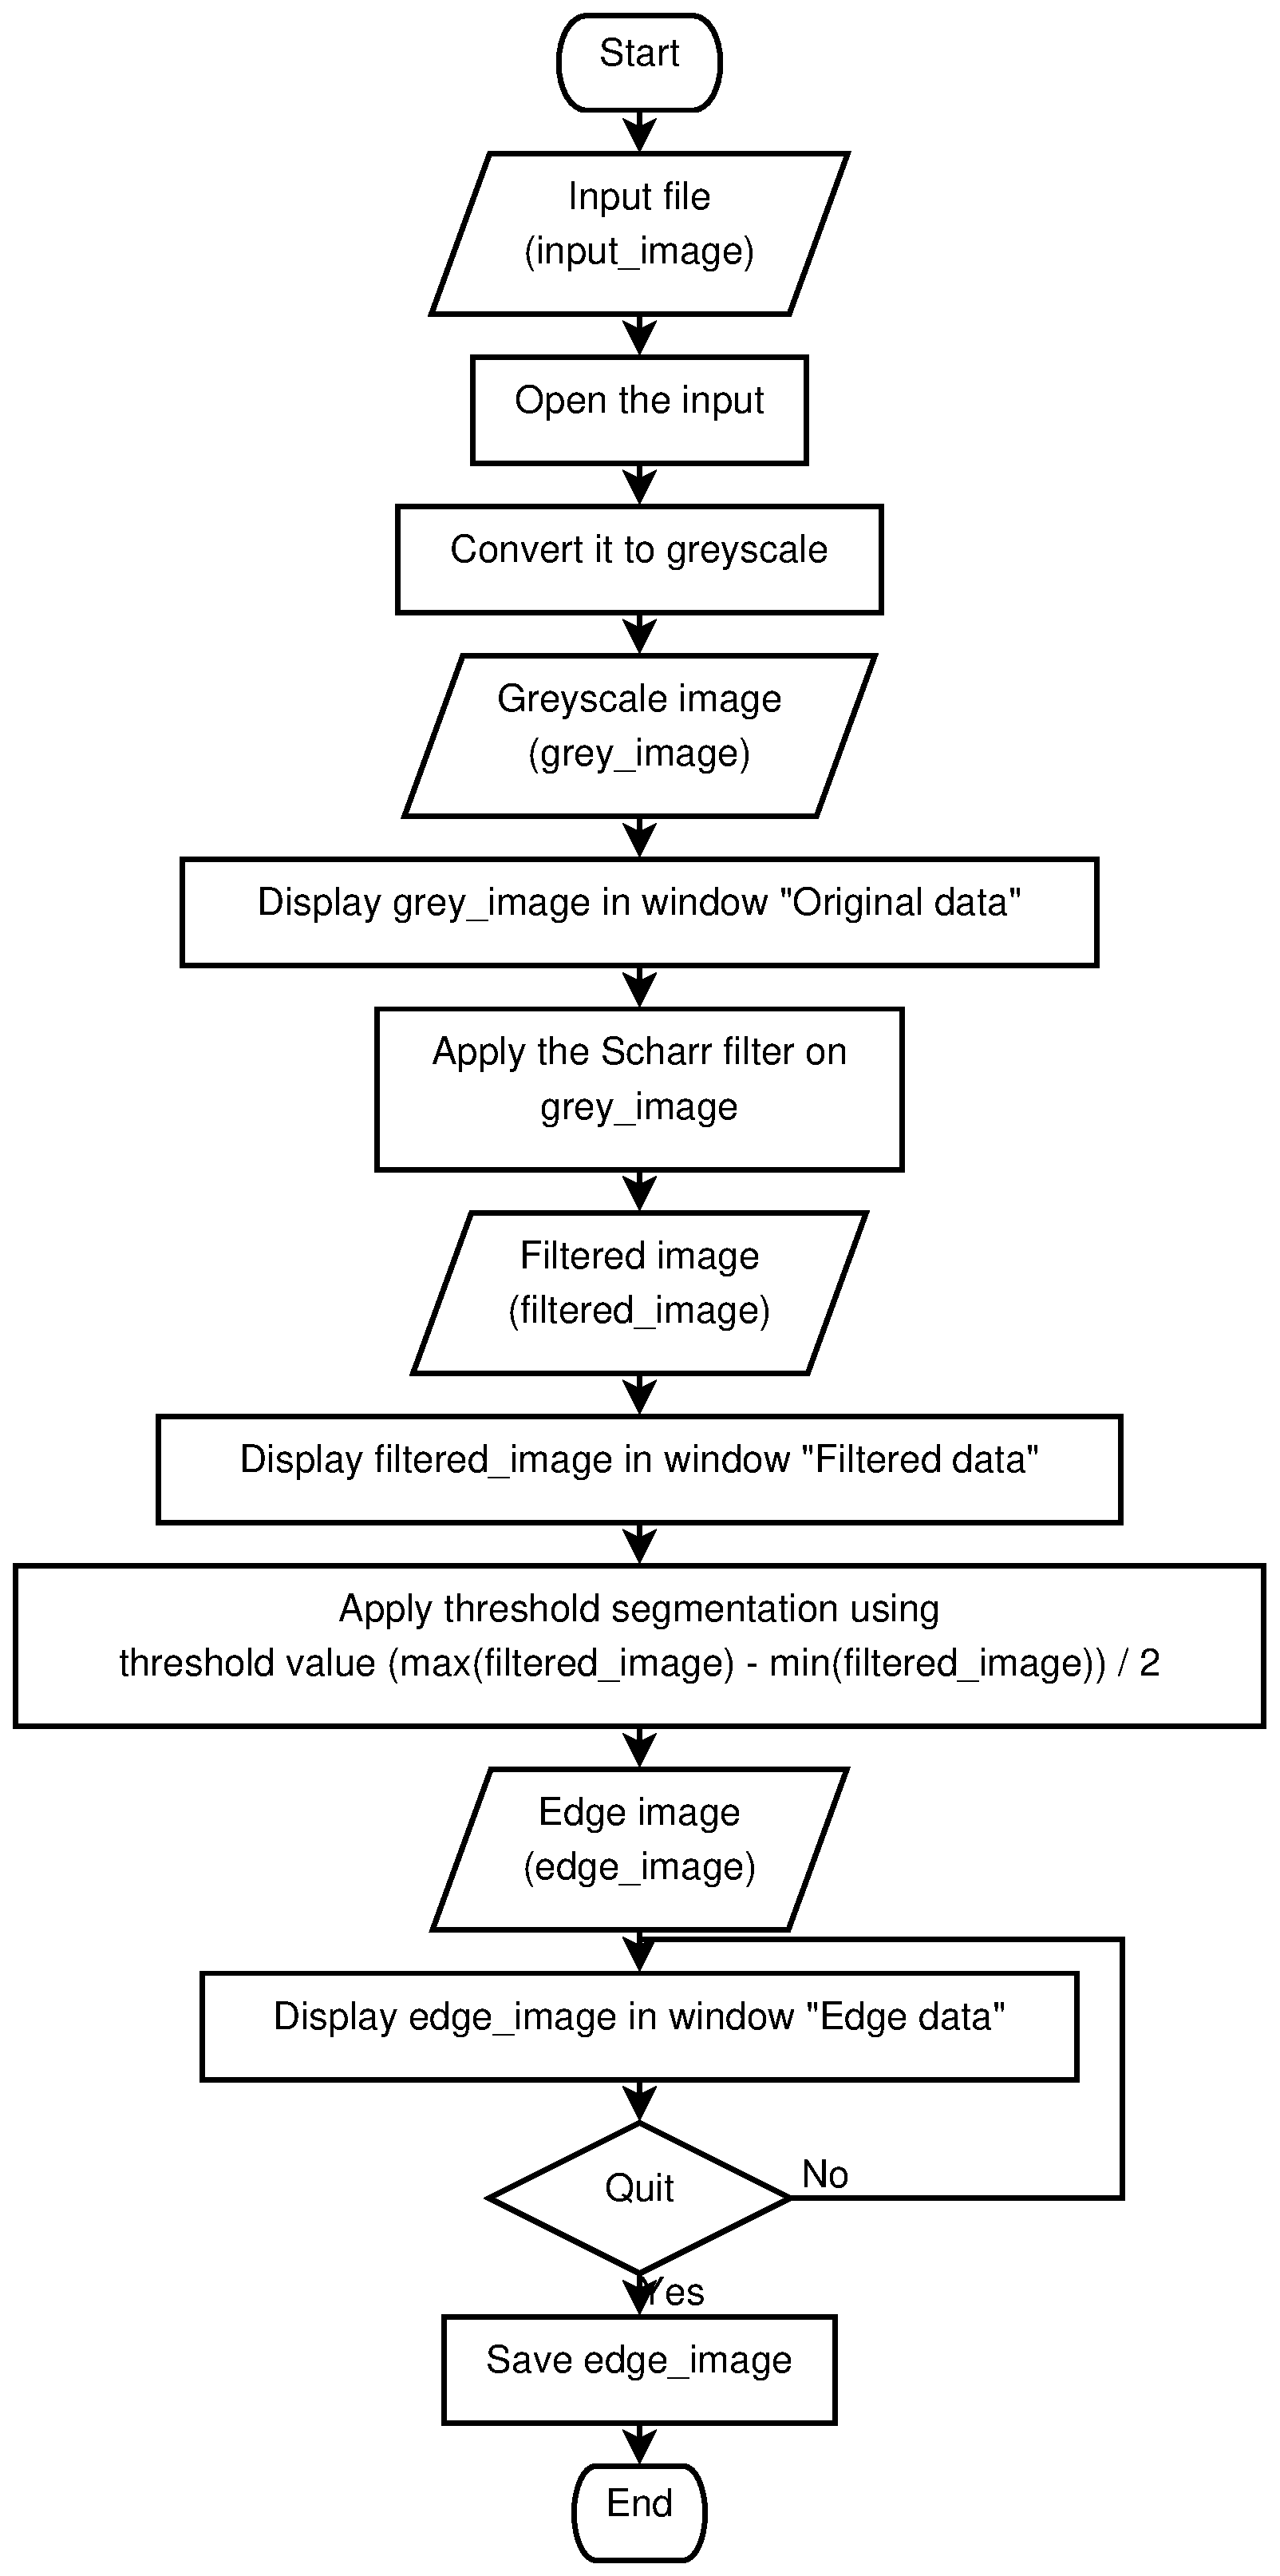
\includegraphics[height=20cm]{flow_chart_edge_detection}
 \caption{\label{fig:flowChart}Flow chart of \emph{edgeDetection1.cxx}.}
\end{figure}
The skeleton of the program is provided, you need to complete it with your own code. 

There are several main steps:
\begin{enumerate}
	\item Declare some local variables;

	\item Read the input;

	\item Convert the RGB data to greyscale:

	\begin{enumerate}
		\item Convert the RGB data to greyscale (see \verb+cv::cvtColor+).
		We did it last week and remember that OpenCV4 is not fully backward compatible with OpenCV3. 
		In OpenCV3, the colour space conversion code is \verb+CV_RGB2GRAY+; in OpenCV4, it is \verb+cv::COLOR_RGB2GRAY+. 
		\item Convert the image from unsigned char to float (see \verb+cv::Mat::convertTo+). 
		Again, we did it last week and remember that OpenCV4 is not fully backward compatible with OpenCV3. 
		\item Normalise the image (see \verb+cv::normalize+) so that the pixel values are in the range between 0 and 1.
		Last week we used \verb+ cv::normalize(log_image, normalised_image, 0, 255,+ \verb+    cv::NORM_MINMAX, CV_8UC1)+ \\
		\verb+CV_8UC1+ means that pixel values in the produced output (\verb+normalised_image+) are stored using unsigned integers with 8 bits (\verb+8U+ in \verb+CV_8UC1+) (i.e.~\verb+unsigned char+ in C/C++), they correspond to luminance values (\verb+C1+ in \verb+CV_8UC1+), and the dynamic range of \verb+normalised_image+ is [0, 255]. 
		This week we will use \verb+ cv::normalize(grey_image, normalised_image, 0.0, 1.0,+ \verb+    cv::NORM_MINMAX, CV_32FC1)+\\ \verb+32F+ in \verb+CV_32FC1+ means \verb+float+ in C/C++.
	\end{enumerate}

	\item Apply a $3 \times 3$ Gaussian filter with $\sigma$ equal to 0.5 to reduce noise (see \verb+cv::GaussianBlur+).

	\item Get the gradient image:
	\begin{enumerate}
		\item Apply the Scharr filter on the blurred image along the X-axis (see \verb+cv::Scharr+);
		\item Compute the absolute value of the gradient along the X-axis (see \verb+cv::abs+);
		\item Apply the Scharr filter on the blurred image along the Y-axis;
		\item Compute the absolute value of the gradient along the Y-axis;
		\item Combine the two images together so that:
		$$gradient(x,y) = 0.5 \times |scharr_x(x,y)| + 0.5 \times |scharr_y(x,y)|$$
		\verb+operator*+ and \verb!operator+! have been overloaded in OpenCV. You can achieve the blending operation using them.
	\end{enumerate}
	\item Find edges using a binary threshold filter (see \verb+cv::threshold+).
	\item Write the output. Remember to normalise the image between 0 and 255 before writing the file. 
\end{enumerate}

Last week, we used:
\begin{itemize}
 \item \verb+cv::cvtColor+ in \verb+rgb2grey.cxx+; 
 \item \verb+cv::Mat::convertTo+ in \verb+rgb2grey.cxx+; 
 \item \verb+cv::normalize+ in \verb+logScale.cxx+; and 
 \item \verb+cv::GaussianBlur+ in \verb+gaussianFilter.cxx+.
\end{itemize}

\subsection{ImageDerivative (High-Pass Filter)}
To calculate the image derivative, you need to call the Scharr operator:
 \begin{lstlisting}[language=c++]
 void cv::Scharr(const cv::Mat& src, cv::Mat& dst, int ddepth, int dx, int dy)
\end{lstlisting}
with:
\begin{description}
 \item[src:] input image;
 \item[dst:] output image of the same size and the same number of channels as \verb+src+;
 \item[ddepth:] output image depth, you can use \verb+CV_32F+;
 \item[dx:] order of the derivative x (= 0 or 1);
 \item[dy:] order of the derivative y (= 0 or 1).
\end{description}

\subsection{Pixel-wise Absolute Value Filter}
To calculate the absolute image of the derivative, you need to call:
 \begin{lstlisting}[language=c++]
 cv::Mat cv::abs(const cv::Mat& src)
\end{lstlisting}
with:
\begin{description}
 \item[src:] input image;
 \item[return:] output image of the same size and the same number of channels as \verb+src+;
\end{description}


\subsection{Binary Threshold Filter}

To calculate the absolute image, so that
$$
dst(x,y)=
\left\lbrace	\begin{array}{ll}
		max\_value & \forall~x~\&~y, \mathrm{if}~src(x,y) > threshold\\
		0 & otherwise
	\end{array}
	\right.
$$
with $max\_value = 1$ in our case as we are dealing with pixel values stored using floating point numbers. 
You need to call:
 \begin{lstlisting}[language=c++]
 cv::Mat cv::threshold(const cv::Mat& src, cv::Mat dst, double threshold, double max_value, int threshold_type)
\end{lstlisting}
with:
\begin{description}
 \item[src:] input image;
 \item[dst:] output image of the same size and the same number of channels as \verb+src+;
 \item[threshold:] the threshold value;
 \item[max\_value:] the maximum value in the output;
 \item[threshold\_type:] the threshold type, here 0 for a binary threshold.
\end{description}

Try different value of threshold to get an acceptable result.



\section{Improve the previous program}

Copy paste some of the code from the \verb+main+ function of \verb+edgeDetection1.cxx+ into \verb+edgeDetection2.cxx+. 
We are going to improve the program. 
Finding the best value of threshold is not easy. 
We can use an adjustable slider to do so. 
Also, we can display the 3 images side by side. 
In other words, we want to create a single window that looks like Figure~\ref{fig:window}. 
\begin{figure}[htbp]
 \centering
 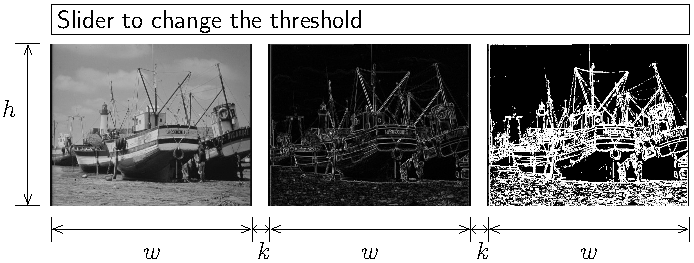
\includegraphics{display}
 \caption{\label{fig:window}User interface. $w$ is the image width in pixels, $h$ is the image height in pixels, and $k$ is the number of empty pixels between two successive images.}
\end{figure}

\subsection{Global variables}
The slider will require a callback function that is why we need to move 
 \begin{lstlisting}[language=c++]
cv::Mat g_scharr_image;
cv::Mat g_edge_image;
std::string g_image_window_title("Edge detection");
\end{lstlisting}
as global variables. 


\subsection{Displayed image}

We also need to create a new image, e.g.~\verb+g_display_image+, as a global variable to hold the data to be displayed. 
Its size is $N \times w + (N - 1) \times k$ with:
 $w$ the image width in pixels, $h$ the image height in pixels, $k$ the number of empty pixels between two successive images, and
 $N$ the number of images displayed in a row.
It is created as follows:
 \begin{lstlisting}[language=c++]
// Create the displayed image
g_display_image = cv::Mat(rgb_image.rows, rgb_image.cols * N + (N - 1) * k, CV_32FC1, cv::Scalar(0.5, 0.5, 0.5));
\end{lstlisting}

Data from the images (\verb+grey_image+, \verb+g_scharr_image+ and \verb+g_edge_image+) will be copied in \verb+g_display_image+. 
To do it, we first need to define the region of interest in the target image, for example with:
 \begin{lstlisting}[language=c++]
// Create the ROI in the target image
cv::Mat targetROI = g_display_image(cv::Rect(offset_x, offset_y, width, height))
\end{lstlisting}
then copy from the source to the target with:
 \begin{lstlisting}[language=c++]
grey_image.copyTo(targetROI);
\end{lstlisting}
\begin{itemize}
 \item For \verb+grey_image+,     \verb+offset_x+ is $0 \times grey\_image.cols + 0 \times k$;
 \item For \verb+g_scharr_image+, \verb+offset_x+ is $1 \times g\_scharr\_image.cols + 2 \times k$; and
 \item For \verb+g_edge_image+,   \verb+offset_x+ is $2 \times g\_edge\_image.cols + 2 \times k$. 
\end{itemize}
\verb+offset_y+ is null.


\subsection{Slider}

The slider is created with:
 \begin{lstlisting}[language=c++]
        cv::createTrackbar(const string& aLabel, const string& aWindowTitle, int* aSliderPosition, int aSliderCount, void (*aCallback)(int, void*));
\end{lstlisting}
\begin{description}
 \item[aLabel:] the text describing the slider;
 \item[aWindowTitle:] the title of the window to which the slider will be attached;
 \item[aSliderPosition:] a pointer on the slider position;
 \item[aSliderCount:] the number of ticks;
 \item[aCallback:] the pointer on the callback function called when the slider moves (in C/C++ it is the name of the function without its parameters).
\end{description}

You can create two global variables such as:
\begin{lstlisting}[language=c++]
int g_slider_count(256);
int g_slider_position(g_slider_count / 2);
\end{lstlisting}
This way, they will be available in the callback function. 
 
 \subsection{Callback}
 
The type of the call back is:
\begin{lstlisting}[language=c++]
void callback(int, void*)
\end{lstlisting}
We do not use the parameters, ignore them.
In the callback there are 4 steps:
\begin{itemize}
 \item Get the threshold from \verb+g_slider_count+ and \verb+g_slider_position+ using linear interpolation.
 \item Compute the new image.
 \item Copy the results in \verb+g_display_image+.
 \item Display \verb+g_display_image+ in the window.
\end{itemize}


\section{Canny edge detector}

We are going to replace the edge detection based on Sharr filtering and thresholding with a dedicated algorithm: the famous Canny operator. 
\begin{lstlisting}[language=c++]
void cv::Canny	(InputArray 	image,
	OutputArray 	edges,
	double 	threshold1,
	double 	threshold2,
	int 	apertureSize = 3,
	bool 	L2gradient = false)		
\end{lstlisting}
\begin{description}
\item[image:] 	8-bit input image.
\item[edges:]	output edge map; single channels 8-bit image, which has the same size as image.
\item[threshold1:]	first threshold for the hysteresis procedure.
\item[threshold2:]	second threshold for the hysteresis procedure.
\item[apertureSize:]	aperture size for the Sobel operator.
\item[L2gradient:]	a flag, indicating whether a more accurate $L_2 norm = \sqrt{\left(\frac{dI}{dx}\right)^2+\left(\frac{dI}{dy}\right)^2}$ should be used to calculate the image gradient magnitude ( L2gradient=true ), or whether the default $L_1 norm = \left|\frac{dI}{dx}\right|+\left|\frac{dI}{dy}\right|$ ( L2gradient=false ).
\end{description}

As you can see, this algorithm requires two threshold values: one low; one high. 
The changes that are required are as follows:
\begin{itemize}
\item In the \verb+main+ function:
    \begin{enumerate}
    \item Move the declaration of \verb+gaussian_image+ so that it becomes a global variable. Rename every occurrence of \verb+gaussian_image+ into \verb+g_gaussian_image+ so that it is clear that it is a global variable (compile and test your code NOW to make sure that it works). 
    \item Delete the global variable \verb+g_slider_position+. As we need two thresholds, we are going to use more meaningful names.
    \item Create a new global variable \verb+g_low_slider_position+. Initialise it to \verb+g_slider_count / 4+.
    \item Create a new global variable \verb+g_high_slider_position+. Initialise it to \verb+g_slider_count / 2+.
    \item Delete the old slider, we are going to need to, one per threshold. 
    \item Create the new sliders (make sure the label are meaningful and use the corresponding slider position variables, i.e. \verb+g_low_slider_position+ and \verb+g_high_slider_position+.
    \end{enumerate}
    \item In the \verb+callback+ function:
        \begin{enumerate}
        \item Update the code of the linear interpolation to find the two thresholds:
         \begin{lstlisting}[language=c++]
double low_threshold(255 * (double(std::min(g_low_slider_position,   g_high_slider_position) / double(g_slider_count))));
double high_threshold(255 * (double(std::max(g_low_slider_position, g_high_slider_position) / double(g_slider_count))));
	\end{lstlisting}
	Note the use of \verb+std::min(a,b)+ and \verb+std::max(a,b)+  to ensure 
	$low\_threshold \leq high\_threshold$. Don't forget the header inclusion. The two functions are defined in Header \verb+<algorithm>+.
	\item Remove the call to \verb+cv::threshold+ as we are replacing it with the Canny operator.
	\item The input of this operator has to be in \verb+unsigned char+ and in luminance (see \verb+CV_8UC1+ below). We create a temporary variable for this purpose:
         \begin{lstlisting}[language=c++]
cv::Mat grey_image;
g_gaussian_image.convertTo(grey_image, CV_8UC1, 255);
	\end{lstlisting}

	\item Call the Canny operator as follows (see the use of the two thresholds):
         \begin{lstlisting}[language=c++]
cv::Canny(grey_image, g_edge_image, low_threshold, high_threshold);
	\end{lstlisting}

	\item Before you use the resulting image, convert it into an image of floating point numbers:
         \begin{lstlisting}[language=c++]
g_edge_image.convertTo(g_edge_image, CV_32FC1, 1.0 / 255.0);
	\end{lstlisting}

    \end{enumerate}

\end{itemize}



%\section{Still some time left?}
%
%If you are done and still have a bit of time, you can look at displaying videos using OpenCV.
%Copy the code of \verb+edgeDetection2.cxx+ into \verb+edgeVideo.cxx+. 
%Checkout \url{http://docs.opencv.org/2.4/modules/highgui/doc/reading_and_writing_images_and_video.html#videocapture} to use a video stream from a file (e.g.~an AVI file) or from the webcam. 


 % 
% 
% 
% Note
% 
% This function should be followed by waitKey function which displays the image for specified milliseconds. Otherwise, it won’t display the image. For example, waitKey(0) will display the window infinitely until any keypress (it is suitable for image display). waitKey(25) will display a frame for 25 ms, after which display will be automatically closed. (If you put it in a loop to read videos, it will display the video frame-by-frame) 
% 
% 
% 
% 
% 
% \subsection{Arguments of the Command Line}
% 
% The first program only takes one parameter. 
% It corresponds to the path of an image file. 
% 
% To make sure the number of arguments is correct, you can use:
% 
%  \begin{lstlisting}[language=c++]
%        // No file to display
%         if (argc != 2)
%         {
%             // Create an error message
%             std::string error_message;
%             error_message  = "usage: ";
%             error_message += argv[0];
%             error_message += " <input_image>";
% 
%             // Throw an error
%             throw error_message;
%         }
% \end{lstlisting}
% 
% \subsection{Reading the File}
% 
% An image is stored in a \verb+Mat+ class instance. 
% Note that OpenCV's namespace is \verb+cv::+. 
% To declare the variable that will hold our image, type:
%  \begin{lstlisting}[language=c++]
%         // Create an image instance
%         cv::Mat image;
% \end{lstlisting}
% 
% The image is loaded using:
%  \begin{lstlisting}[language=c++]
%         // Open and read the image
%         image = cv::imread( argv[1], CV_LOAD_IMAGE_COLOR );
% \end{lstlisting}
% 
% It is a good practice to check if any error occurred, e.g.~to avoid unspecified behaviours and crashed. 
% If the image is not loaded, its \verb+data+ field is empty. 
% If it is the case we can throw an error as follows:
%  \begin{lstlisting}[language=c++]
%         // The image has not been loaded
%         if (!image.data)
%         {
%             // Create an error message
%             std::string error_message;
%             error_message  = "Could not open or find the image \"";
%             error_message += argv[1];
%             error_message += "\".";
% 
%             // Throw an error
%             throw error_message;
%         }
% \end{lstlisting}
% 
% 
% \subsection{Displaying the Image}
% 
% There are four steps to create a window and display and image:
% \begin{enumerate}
%  \item Create a string to contain the window title;
%  \item Create the window;
%  \item Show the image in the window;
%  \item Wait for a user input to leave the window.
% \end{enumerate}
% 
% It can be done as follows:
% \begin{lstlisting}[language=c++]
%         // Create a string to contain the window title
%         string window_title;
%         window_title  = "Display \"";
%         window_title += argv[1];
%         window_title += "\"";
% 
%         // Create the window
%         cv::namedWindow(window_title, cv::WINDOW_AUTOSIZE);
% 
%         // Show the image in the window
%         cv::imshow(window_title, image);
% 
%         // Wait for a user input to leave the window
%         cv::waitKey(0);
% \end{lstlisting}
% 
% The program is now complete. 
% You can compile it and run it with different image files to test it.
% 
% 
% %%%%%%%%%%%%%%%%%%%%%%%%%%%%%%%%%%%%%%%%%%%%%%%%%%%%%%%%%%%%%%%%%%%%%%%%%%%%%%%%
% \section{Convert a RGB Image in a Greyscale Image}
% 
% Copy the code of \verb+DisplayImage.cxx+ in \verb+rgb2grey.cxx+.
% 
% \subsection{Arguments of the Command Line}
% 
% The second program takes two parameter:
% \begin{enumerate}
%  \item  The path of the input RGB image file, and
%  \item  The path of the output greyscale image file.
% \end{enumerate}
% Modify the code accordingly. 
% 
% 
% \subsection{Converting from RGB to Greyscale}
% 
% After displaying the RGB image and BEFORE \verb+cv::waitKey(0)+, create a new image called \verb+grey_image+. 
% To convert the original image in greyscale, simply type:
% \begin{lstlisting}[language=c++]
%         // If the image is not a greyscale image, then convert it.
%         cv::cvtColor(image, grey_image, CV_RGB2GRAY);
% \end{lstlisting}
% 
% In OpenCV in general, the first argument is the input image; the second argument is the output image; other arguments are the parameters of the function. 
% Now create another window where to display the new image. 
% 
% \subsection{Saving an Image into a File}
% 
% The function to save an image is \verb+cv::imwrite(file_name, image)+. 
% It returns true if the file has been successfully written; false otherwise. 
% We can use the return value to handle possible errors:
% \begin{lstlisting}[language=c++]
%         // Write the image
%         if (!cv::imwrite(argv[2], grey_image))
%         {
%             // The image has not been written
% 
%             // Create an error message
%             std::string error_message;
%             error_message  = "Could not write the image \"";
%             error_message += argv[2];
%             error_message += "\".";
% 
%             // Throw an error
%             throw error_message;
%         }
% \end{lstlisting}

% 
% %%%%%%%%%%%%%%%%%%%%%%%%%%%%%%%%%%%%%%%%%%%%%%%%%%%%%%%%%%%%%%%%%%%%%%%%%%%%%%%%
% \section{Display an Image in the Log Scale}
% 
% Copy the code of \verb+rgb2grey.cxx+ in \verb+logScale.cxx+.
% Fig.~\ref{fig:log} shows the shape of the $\log$ function. 
%     \begin {figure}[htb]
%       \begin{center}
%         \input{log}
%       \end{center}
%       \caption{\label{fig:log}The $\log$ function.}
%     \end {figure}
% Looking at the $y$ axis, we note that we need to store the image using floating point numbers. 
% If we don't, we will have enormous quantisation problems. 
% 
% To convert the greyscale image in \verb+unsigned char+ to \verb+float+, we use:
% \begin{lstlisting}[language=c++]
%         // Convert to float
%         cv::Mat float_image;
%         grey_image.convertTo(float_image, CV_32FC1);
% \end{lstlisting}
% 
% It can be seen on the figure that $\log(x) \forall x \in ]-\infty,  0]$ is undefined. 
% In other word, if $x$ is equal to zero or $x$ is negative, then there is no $y$ value. 
% As the input image was using \verb+unsigned char+, we do not have to worry about negative values. 
% However, we have to make sure no $0$ value is present in the image. 
% To do so, we apply the following transformation:
% \begin{equation}f'(x,y) = \log(f(x,y) + 1)\end{equation}
% using
% \begin{lstlisting}[language=c++]
%         // Log transformation
%         cv::Mat log_image;
%         cv::log(float_image + 1.0, log_image);
% \end{lstlisting}
% 
% Looking at the curve, we notice another problem. 
% In some case, $\log(x)$ may be negative. 
% In this case, it is common to normalise the image so that its values lie in the range $[0, 1]$ using:
% \begin{equation}f''(x,y) = \frac{f'(x,y) - \min(f')}{\max(f') - \min(f')}\label{eq:normal}\end{equation}
% 
% There are two ways to achieve this in OpenCV.
% You can implement Eq.~\ref{eq:normal} using:
% \begin{lstlisting}[language=c++]
%         double min, max;
%         cv::minMaxLoc(log_image, &min, &max);
%         cv::Mat normalised_image = (log_image - min) / (max - min);
% \end{lstlisting}
% or you can use OpenCV's function:
% \begin{lstlisting}[language=c++]
%         // Normalisation
%         cv::Mat normalised_image;
%         cv::normalize(log_image, normalised_image, 0.0, 1.0, cv::NORM_MINMAX, CV_32FC1);
% \end{lstlisting}
% 
% Now you can display the image.
%     
% 
% %%%%%%%%%%%%%%%%%%%%%%%%%%%%%%%%%%%%%%%%%%%%%%%%%%%%%%%%%%%%%%%%%%%%%%%%%%%%%%%%
% \section{Mean Filter}
% 
% Now you can perform pixel-wise operations, such as \verb+float_image + 1.0+ or \verb+cv::log(...)+, we can look at filtering images. 
% First, let us consider the mean filter. 
% In this case, the program will take 3 inputs: 
% \begin{enumerate}
%     \item The input image;
%     \item The output image; and
%     \item The convolution kernel radius.
% \end{enumerate}
% To convert a C string into an integer, use the \verb+atoi+ function from \verb+include <cstdlib>+. 
% It will be need to get the kernel radius from the command line argument. 
% To set the kernel size, you need to use an instance of the \verb+cv::Size+ class. 
% You also have to specify its size. 
% You can use:
% \begin{lstlisting}[language=c++]
%         // Filter size
%         cv::Size filter_size(kernel_width, kernel_height);
% \end{lstlisting}
% or 
% \begin{lstlisting}[language=c++]
%         // Filter size
%         cv::Size filter_size;
%         filter_size.width = kernel_width;
%         filter_size.height = kernel_height;
% \end{lstlisting}
% Note that 
% \begin{itemize}
% 	\item If the radius is 0, then the kernel size is $1\times1$    
% 	\item If the radius is 1, then the kernel size is $3\times3$    
% 	\item If the radius is 2, then the kernel size is $5\times5$    
% 	\item ...
% 	\item If the radius is 7, then the kernel size is $15\times15$    
% 	\item etc.
% \end{itemize}
% Now you are ready to filter the input image. Use either \verb+cv::blur+ or \verb+cv::boxFilter+. 
% They are the same. 
% The first argument is the input image; the second is the output image; and the third one is the kernel size. 
% Display and save the output image. 
% Try different kernel sizes to see the differences. 
% 
%         
% %%%%%%%%%%%%%%%%%%%%%%%%%%%%%%%%%%%%%%%%%%%%%%%%%%%%%%%%%%%%%%%%%%%%%%%%%%%%%%%%
% \section{Median Filter}
% 
% You can also use a median filter. 
% In this can, no instance of  \verb+cv::Size+ is required. 
% Just use \verb+cv::medianBlur+. 
% The first argument is the input image; the second is the output image; and the third one is an odd number which corresponds to the kernel size. 
% Try different kernel sizes to see the differences. 
% 
%         
% %%%%%%%%%%%%%%%%%%%%%%%%%%%%%%%%%%%%%%%%%%%%%%%%%%%%%%%%%%%%%%%%%%%%%%%%%%%%%%%%
% \section{Gaussian Filter}
% 
% Finally, let us try the Gaussian filter. 
% You will need 4 parameters from the command line:
% input file, output file, kernel radius and $\sigma$.
% Just like the mean filter, an instance of \verb+cv::Size+ is needed as the Gaussian filter is a convolution. 
% The first three parameters of \verb+cv::GaussianBlur+ are consistent. 
% The fourth and fifth are the horizontal and vertical $\sigma$ values. 
% Try different kernel sizes and different  $\sigma$ values to see the differences. 
% 

%%%%%%%%%%%%%%%%%%%%%%%%%%%%%%%%%%%%%%%%%%%%%%%%%%%%%%%%%%%%%%%%%%%%%%%%%%%%%%%%
\end{document}
